% uOttawa (unofficial) Thesis Template for LaTeX 
% Edited by Wail Gueaieb based on Stephen Carr's uWaterloo Template

% The files included in this package are slighly modified by Suruz Miah to adapt partial requirements  in writing project/thesis reports of the Bradley University's Department of Electrical and Computer Engineering.

% DON'T USE THIS TEMPLATE IF YOU DON'T KNOW WHAT YOU'RE DOING!
% Remember, it comes WITH NO WARRANTY!

% Please read the "00readme.txt" file first.
% Here is how to use this template:
%
% DON'T FORGET TO ADD YOUR OWN NAME AND TITLE in the "hyperref" package
% configuration in the "thesis-preample.tex" file. THIS INFORMATION GETS 
% EMBEDDED IN THE PDF FINAL PDF DOCUMENT.
% You can view the information if you view Properties of the PDF document.

% The template is based on the standard "book" document class which provides 
% all necessary sectioning structures and allows multi-part theses.

% DISCLAIMER
% To the best of our knowledge, this template satisfies the current 
% uOttawa thesis requirements.
% However, it is your responsibility to assure that you have met all 
% requirements of the university and your particular department.
% Many thanks to the feedback from many graduates that assisted the 
% development of this template.

% -----------------------------------------------------------------------

% When using pdflatex, by default the output is geared toward generating a PDF 
% version optimized for viewing on an electronic display, including 
% hyperlinks within the PDF.
 
% E.g. to process a thesis based on this template, run:

% (pdf)latex thesisMain	-- first pass of the (pdf)latex processor
% bibtex thesisMain 	-- generates bibliography from .bib data file(s) 
% (pdf)latex thesisMain	-- fixes cross-references, bibliographic references, etc
% (pdf)latex thesisMain	-- fixes cross-references, bibliographic references, etc
% makeindex -s nomentbl.ist -o thesisMain.nls thesisMain.nlo
% (pdf)latex thesisMain	-- fixes cross-references, bibliographic references, etc
% (pdf)latex thesisMain	-- fixes cross-references, bibliographic references, etc



% N.B. The "pdftex" program allows graphics in the following formats to be
% included with the "\includegraphics" command: PNG, PDF, JPEG, TIFF
% Tip 1: Generate your figures and photos in the size you want them to appear
% in your thesis, rather than scaling them with \includegraphics options.
% Tip 2: Any drawings you do should be in scalable vector graphic formats:
% SVG, PNG, WMF, EPS and then converted to PNG or PDF, so they are scalable in
% the final PDF as well.
% Tip 3: Photographs should be cropped and compressed so as not to be too large.

% To create a PDF output that is optimized for double-sided printing: 
%
% 1) comment-out the \documentclass statement in the preamble below, and
% un-comment the second \documentclass line.
%
% 2) change the value assigned below to the boolean variable
% "PrintVersion" from "false" to "true".

% --------------------- Start of Document Preamble -----------------------

% Specify the document class, default style attributes, and page dimensions
% For hyperlinked PDF, suitable for viewing on a computer, use this:
% \UseRawInputEncoding

% \documentclass[letterpaper,12pt,titlepage,oneside,final]{book}
 
% For PDF, suitable for double-sided printing, change the PrintVersion variable below
% to "true" and use this \documentclass line instead of the one above:
\documentclass[letterpaper,12pt,titlepage,openright,twoside,final]{book}


% This package allows if-then-else control structures.
\usepackage{ifthen}
\newboolean{PrintVersion}
\setboolean{PrintVersion}{false} 
% \setboolean{PrintVersion}{true} 
% CHANGE THIS VALUE TO "true" as necessary, to improve printed results 
% for hard copies by overriding some options of the hyperref package.

%%%%%%%%%%%%%%%%%%%%%
% MATLAB Code
\usepackage[framed,numbered,autolinebreaks,useliterate]{mcode}
%%%%%%%%%%%%%%%%%%%%%

%%%%%%%%%%%%%%%%%%%%%
% Algorithm 
\usepackage[english,algo2e,algoruled,vlined,linesnumbered]{algorithm2e}
%%%%%%%%%%%%%%%%%%%%%

%%%%%%%%%%%%%%%%%%%%%
% Table
\usepackage{booktabs}
%%%%%%%%%%%%%%%%%%%%%

%%%%%%%%%%%%%%%%%%%%%
% Enable Subfigures
\usepackage{caption}
\usepackage{subcaption}
%%%%%%%%%%%%%%%%%%%%%

%%%%%%%%%%%%%%%%%%%%%
% Enable todonotes
\usepackage{todonotes}
%%%%%%%%%%%%%%%%%%%%%

% Load your needed packages and other commands of yours.
% Load your needed packages and other commands of yours here:
%\usepackage{} % ... note that old .sty files can be included here

















%--------------------------------------------------------------------------
% Do NOT edit the rest of the preample UNLESS YOU KNOW WHAT YOU'RE DOING!
%--------------------------------------------------------------------------

\ifthenelse{\boolean{PrintVersion}}{
\usepackage[top=1in,bottom=1in,left=0.75in,right=1.25in]{geometry}   % For twoside document
}{
\usepackage[top=1in,bottom=1in,left=0.75in,right=1.25in]{geometry}   % For oneside document
}

\usepackage{amsmath,amssymb,amstext} % Lots of math symbols and environments
\usepackage{graphicx} % For including graphics 

\usepackage{nomentbl} 
\makenomenclature 

\usepackage{ifpdf}

\newcommand{\href}[1]{#1} % does nothing, but defines the command so the
    % print-optimized version will ignore \href tags (redefined by hyperref pkg).
%\newcommand{\texorpdfstring}[2]{#1} % does nothing, but defines the command
% Anything defined here may be redefined by packages added below...


% Hyperlinks make it very easy to navigate an electronic document.
% In addition, this is where you should specify the thesis title
% and author as they appear in the properties of the PDF document.
% Use the "hyperref" package 
% N.B. HYPERREF MUST BE THE LAST PACKAGE LOADED; ADD ADDITIONAL PKGS ABOVE
\usepackage[\ifpdf pdftex,\fi letterpaper=true,pagebackref=false]{hyperref} % with basic options
		% N.B. pagebackref=true provides links back from the References to the body text. This can cause trouble for printing.
\hypersetup{
    plainpages=false,       % needed if Roman numbers in frontpages
    pdfpagelabels=true,     % adds page number as label in Acrobat's page count
    bookmarks=true,         % show bookmarks bar?
    unicode=false,          % non-Latin characters in Acrobat's bookmarks
    pdftoolbar=true,        % show Acrobat's toolbar?
    pdfmenubar=true,        % show Acrobat's menu?
    pdffitwindow=false,     % window fit to page when opened
    pdfstartview={FitH},    % fits the width of the page to the window
%    pdftitle={uOttawa\ LaTeX\ Thesis\ Template},    % title: CHANGE THIS TEXT!
%    pdfauthor={Author},    % author: CHANGE THIS TEXT! and uncomment this line
%    pdfsubject={Subject},  % subject: CHANGE THIS TEXT! and uncomment this line
%    pdfkeywords={keyword1} {key2} {key3}, % list of keywords, and uncomment this line if desired
    pdfnewwindow=true,      % links in new window
    colorlinks=true,        % false: boxed links; true: colored links
    linkcolor=blue,         % color of internal links
    citecolor=green,        % color of links to bibliography
    filecolor=magenta,      % color of file links
    urlcolor=cyan           % color of external links
}
\ifthenelse{\boolean{PrintVersion}}{   % for improved print quality, change some hyperref options
\hypersetup{	% override some previously defined hyperref options
%    colorlinks,%
    citecolor=black,%
    filecolor=black,%
    linkcolor=black,%
    urlcolor=black}
}{} % end of ifthenelse (no else)

\usepackage{fancyhdr,lastpage} % Change caption style; changes headers and page styles etc.
\usepackage{epstopdf}
\epstopdfsetup{suffix={}}


% This is where thesis margins and spaces are set.
% Setting up the page margins...
% A minimum of 1 inch (72pt) margin at the
% top, bottom, and outside page edges and a 1.125 in. (81pt) gutter
% margin (on binding side). While this is not an issue for electronic
% viewing, a PDF may be printed, and so we have the same page layout for
% both printed and electronic versions, we leave the gutter margin in.
% Set margins:
\setlength{\marginparwidth}{0pt} % width of margin notes
% N.B. If margin notes are used, you must adjust \textwidth, \marginparwidth
% and \marginparsep so that the space left between the margin notes and page
% edge is less than 15 mm (0.6 in.)
\setlength{\marginparsep}{0pt} % width of space between body text and margin notes
\setlength{\evensidemargin}{0.125in} % Adds 1/8 in. to binding side of all 
% even-numbered pages when the "twoside" printing option is selected
\setlength{\oddsidemargin}{0.125in} % Adds 1/8 in. to the left of all pages
% when "oneside" printing is selected, and to the left of all odd-numbered
% pages when "twoside" printing is selected
\setlength{\textwidth}{6.375in} % assuming US letter paper (8.5 in. x 11 in.) and 
% side margins as above
\raggedbottom

% The following statement specifies the amount of space between
% paragraphs. Other reasonable specifications are \bigskipamount and \smallskipamount.
\setlength{\parskip}{\medskipamount}

% The following statement controls the line spacing.  The default
% spacing corresponds to good typographic conventions and only slight
% changes (e.g., perhaps "1.2"), if any, should be made.
\renewcommand{\baselinestretch}{1} % this is the default line space setting

% By default, each chapter will start on a recto (right-hand side)
% page.  We also force each section of the front pages to start on 
% a recto page by inserting \cleardoublepage commands.
% In many cases, this will require that the verso page be
% blank and, while it should be counted, a page number should not be
% printed.  The following statements ensure a page number is not
% printed on an otherwise blank verso page.
\let\origdoublepage\cleardoublepage
\newcommand{\clearemptydoublepage}{%
  \clearpage{\pagestyle{empty}\origdoublepage}}
\let\cleardoublepage\clearemptydoublepage



\fancypagestyle{myFancy}{%
  \fancyhf{}% Clear header and footer
  \fancyhead[LE,RO]{\bfseries\nouppercase{\rightmark}}
  \fancyhead[LO,RE]{\bfseries\nouppercase{\leftmark}}
  \fancyfoot[R]{Page \thepage\ of \pageref{LastPage}}% Custom footer
  \fancyfoot[L]{K.~Allen, D.~Beebe \& J.~Braker (\nameOfUniversity)}% Custom footer
  \renewcommand{\headrulewidth}{0.4pt}% Line at the header visible
  \renewcommand{\footrulewidth}{0.1pt}% Line at the footer visible
}


%======================================================================
%   L O G I C A L    D O C U M E N T -- the content of your thesis
%======================================================================
\begin{document}
\captionsetup[figure]{labelfont={bf},labelformat={default},labelsep=period,name={Fig.}}
\captionsetup[table]{labelfont={bf},labelformat={default},labelsep=period,name={Tab.}}
% For a large document, it is a good idea to divide your thesis
% into several files, each one containing one chapter.
% To illustrate this idea, the "front pages" (i.e., title page,
% declaration, borrowers' page, abstract, acknowledgements,
% dedication, table of contents, list of tables, list of figures,
% nomenclature).
%----------------------------------------------------------------------
% FRONT MATERIAL
%----------------------------------------------------------------------
%
% C O V E R  P A G E
% ------------------
\newcommand{\thesisauthor}{Kallistah Allen, Darrah Beebe, and Jason Braker}
\newcommand{\advisor}{Dr. Suruz Miah and Dr. Prasad Shastry}
\newcommand{\thesistitlecoverpage}{%
Robotic Cart System
}
%\newcommand{\degree}{Ph.D.} % possible values are:
                            % M.A. / M.A.Sc. / M.Sc. / MCS / Ph.D.
\newcommand{\nameofprogram}{Electrical and Computer Engineering Department}
\newcommand{\academicunit}{Caterpillar College of Engineering and Technology}
%\newcommand{\faculty}{Faculty of Engineering}
\newcommand{\nameOfUniversity}{Bradley University}
\newcommand{\graduationyear}{2021}
%
% T I T L E   P A G E
% -------------------
% Last updated May 24, 2011, by Stephen Carr, IST-Client Services
% The title page is counted as page `i' but we need to suppress the
% page number.  We also don't want any headers or footers.
\pagestyle{empty}
\pagenumbering{roman}

% The contents of the title page are specified in the "titlepage"
% environment.
\begin{titlepage}
        \begin{center}
        \vspace*{1.0cm}

        \Huge
        {\bf \thesistitlecoverpage }

        \vspace*{1.0cm}

        \normalsize
        by \\

        \vspace*{1.0cm}

        \Large
        \thesisauthor\\
        Advisor:~\advisor\\

        \vspace*{3.0cm}

        % \normalsize
        % Thesis submitted to the\\
        % Faculty of Graduate and Postdoctoral Studies\\
        % In partial fulfillment of the requirements\\
        % For the \degree~degree in\\
        % \nameofprogram\\

        \vspace*{2.0cm}

        \nameofprogram\\
        \academicunit\\
        %\faculty\\
        \nameOfUniversity\\

        \vspace*{4.0cm}

        \copyright~\thesisauthor, Peoria, Illinois, \graduationyear\\
        \end{center}
\end{titlepage}

% The rest of the front pages should contain no headers and be numbered using Roman numerals starting with `ii'
% PRELIMINARY PAGES

\pagestyle{plain}
\setcounter{page}{2}

\cleardoublepage % Ends the current page and causes all figures and tables that have so far appeared in the input to be printed.
% In a two-sided printing style, it also makes the next page a right-hand (odd-numbered) page, producing a blank page if necessary.



%%% Local Variables:
%%% mode: latex
%%% TeX-master: "../thesisMain"
%%% End:




%
% R E S T  O F  F R O N T  P A G E S
% ----------------------------------
% % D E C L A R A T I O N   P A G E
% -------------------------------
  % This page is not needed for a uOttawa thesis. Don't include it.
  % It is designed for an electronic thesis.
  \noindent
I hereby declare that I am the sole author of this thesis. This is a true copy of the thesis, including any required final revisions, as accepted by my examiners.

  \bigskip
  
  \noindent
I understand that my thesis may be made electronically available to the public.

\cleardoublepage
%\newpage
 %This is not needed in a uOttawa thesis.
%
% Edit the following 3 files with your abstract, acknowledgements, 
% and dedication.
% A B S T R A C T
% ---------------

\begin{center}\textbf{Abstract}\end{center}

%This paper proposes a strategy for testing and comparing three control algorithms, LQR, LQG, and ADP, to control two two-DOF helicopters from a mobile device.  We will be using Raspberry Pi 3's as terminals for the wireless communication and MATLAB as our primary coding language.

This project proposes a modular and cost-effective smart real-time motion control
framework for a group of two degrees of freedom (2-DOF) helicopters.  The helicopters are
controlled by a mobile device which sends position signals over a wireless network to a
microcontroller.  The microcontroller uses control algorithms to determine the amount of voltage
to apply to DC motors.  This project tests and compares three control algorithms, LQR, LQG, and
ADP as well as theorizes possible methods to improve the control in future projects.

\cleardoublepage
%\newpage


%%% Local Variables:
%%% mode: latex
%%% TeX-master: "../finalReportMainV1"
%%% End:

% A C K N O W L E D G E M E N T S
% -------------------------------

\begin{center}\textbf{Acknowledgements}\end{center}

    \par Special thanks to Mr. Christopher Mattus for his assistance in procuring the parts and modifying 		\par the hardware for our project.
    \par Special thanks to Shreel Patel for his assistance with charging the battery on the robot.
    \par Thank you to everyone else who helped make this project possible and successful.


\cleardoublepage
%\newpage



%%% Local Variables:
%%% mode: latex
%%% TeX-master: "../finalReportMainV1"
%%% End:

% D E D I C A T I O N
% -------------------

\begin{center}\textbf{Dedication}\end{center}

This is dedicated to our loved ones and friends who supported us through our time working on this project.

\cleardoublepage
%\newpage


%%% Local Variables:
%%% mode: latex
%%% TeX-master: "../finalReportMainV1"
%%% End:

%
%
% No need to edit this file.
% T A B L E   O F   C O N T E N T S
% ---------------------------------
\renewcommand\contentsname{Table of Contents}
\tableofcontents
\cleardoublepage
\phantomsection
%\newpage

% L I S T   O F   T A B L E S
% ---------------------------
\addcontentsline{toc}{chapter}{List of Tables}
\listoftables
\cleardoublepage
\phantomsection		% allows hyperref to link to the correct page
%\newpage

% L I S T   O F   F I G U R E S
% -----------------------------
\addcontentsline{toc}{chapter}{List of Figures}
\listoffigures
\cleardoublepage
\phantomsection		% allows hyperref to link to the correct page
%\newpage


%
% No need to edit this file. But you may want to comment the whole line if you
% don't have or want a Nomenclature section.
% L I S T   O F   S Y M B O L S
% -----------------------------
% To include a Nomenclature section
\addcontentsline{toc}{chapter}{\textbf{Nomenclature}}

\renewcommand{\nomname}{Nomenclature}
\renewcommand{\nomAname}{\textbf{\large Abbreviations}}
\renewcommand{\nomGname}{\textbf{\large Mathematical Symbols}}
\renewcommand{\nomXname}{\textbf{\large Superscripts}}
\renewcommand{\nomZname}{\textbf{\large Subscripts}}

\printnomenclature
\cleardoublepage
\phantomsection % allows hyperref to link to the correct page
% \newpage


\nomAname
\begin{itemize}
    \item[]\textbf{RF} - Radio Frequency
    \item[]\textbf{LoS} - Line of Sight
    \item[]\textbf{DDMR} - Differential Drive Mobile Robot
      
\end{itemize}
\bigbreak

\nomGname
\begin{itemize}
	\item[]$\omega_l$ - left angular wheel speed
	\item[]$\omega_r$ - right angular wheel speed
	\item[]$v$ - linear speed
	\item[]$d_(follow)$ - fixed following distance 
    \item[]$K_v$ - proportional gain for linear velocity
    \item[]$K_\omega$ - proportional gain for angular velocity
    \item[]$\theta_r$ - angle of the remote with respect to robot
    \item[]$d_r$ - distance from robot to remote
    \item[]$d_(tgt)$ - distance to the target point

\end{itemize}


%%% Local Variables:
%%% mode: latex
%%% TeX-master: "../finalReport"
%%% End:
  


% Change page numbering back to Arabic numerals
\pagenumbering{arabic}



%

% Redefine the plain page style
\fancypagestyle{plain}{%
  \fancyhf{}%
  \fancyfoot[R]{Page \thepage\ of \pageref{LastPage}}%
  \fancyfoot[L]{K.~Allen, D.~Beebe \& J.~Braker (\nameOfUniversity)}%  
  \renewcommand{\headrulewidth}{0pt}% Line at the header invisible
  \renewcommand{\footrulewidth}{0.1pt}% Line at the footer visible
}
\pagestyle{myFancy}


%----------------------------------------------------------------------
% MAIN BODY
%---------------------------------------------------------------------- 
% Chapters 
% Include your "sub" source files here (must have extension .tex)
%======================================================================
\chapter{Introduction}
\label{ch: Chapter1}
%======================================================================

%----------------------------------------------------------------------
\section{Motivation and Problem Statement}
%----------------------------------------------------------------------
Robotic carts are a prevalent invention designed to aid users in a number of important indoor and outdoor tasks. There are robotic systems currently available in the market that perform these tasks in a variety of ways. For example, in a grocery store, a customer may require the need of more than one cart but cannot push or pull two carts simultaneously. One major drawback, however, is that people with disabilities cannot push one cart let alone have a second cart to carry more items. Moreover, robots used for this purpose are more costly than they are worth.

\vspace*{12pt}
\noindent
In this project, we are proposing a robotic cart that would primarily use analog signals with the use of cost-effective wireless communication to identify the customer and be able to track and follow the customer through the store. The implementation of such a fully functional robotic cart will outreach the scope of the project but is the overall goal for this project in the coming years while encouraging further research in this field.

\vspace*{12pt}
\noindent
Applications of the proposed robotic cart include, but are not limited to, delivery carts to follow mail personnel and carry the deliveries, file transfer carts in offices, hospital carts to aid nurses and doctors by carrying medicine or surgery supplies, and carts in construction sites to carry tools and other supplies across the job site.



%----------------------------------------------------------------------
\section{Literature Review}
%----------------------------------------------------------------------
Abundant research in the field of mobile robotics shows various ways to develop robotic carts that will help consumers in carrying groceries through stores~\cite{Rawashdeh2017-Person,islam_lam_fukuda_kobayashi_kuno_2019,Sales2016-CompaRob}. Currently, the work being done focuses on a few different methods of having a robotic cart interface with the customer and follow them through the store.

\vspace*{12pt}
\noindent
One such method, shown in Fig. \ref{fig:CompaRob}, that has been utilized to make a mobile cart follow a customer through a store is a mobile platform interface that implements ultrasound and radio transmissions technology~\cite{Sales2016-CompaRob}. Another method, shown in Fig. \ref{fig:ShoppingSup}, that has been implemented is the use of a GRU (Gated Recurrent Unit) network to detect shopping habits of customers while also using a LiDAR (Light Detection and Ranging) sensor and camera to detect and map the customer using a two-dimensional skeleton and follow the customer through the store~\cite{islam_lam_fukuda_kobayashi_kuno_2019}. Therein, in Fig. \ref{fig:SmartCart}, authors utilized an Arduino MEGA 2560, six ultrasonic sensors, two DC motors with PWM (Pulse Width Modulation), an Android Studio IDE device, and Bluetooth for detecting a customer and following them through the store~\cite{Rawashdeh2017-Person}.

\begin{figure}[b]
   \centering
   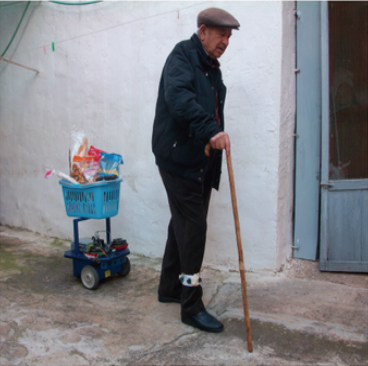
\includegraphics[width=0.4\textwidth]{figs/img/CompaRob}
   \caption{CompaRob Robot}
   \label{fig:CompaRob}
\end{figure}

\begin{figure}[b]
   \centering
   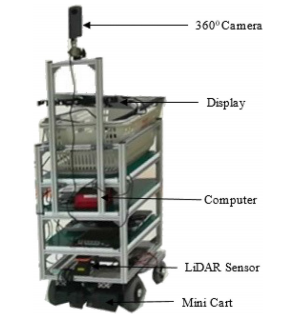
\includegraphics[width=0.38\textwidth]{figs/img/ShoppingSuportRobot}
   \caption{Shopping Support Robot}
   \label{fig:ShoppingSup}
\end{figure}

\begin{figure}[b]
   \centering
   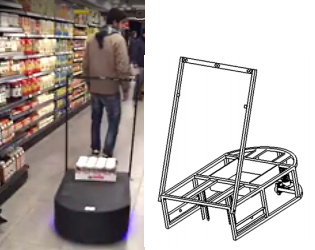
\includegraphics[width=0.45\textwidth]{figs/img/SmartCart}
   \caption{Smart Cart Robot}
   \label{fig:SmartCart}
\end{figure}

\vspace*{12pt}
\noindent
In the current project, we are implementing XBee S2C RF radios, which are inexpensive and easily configurable, as a remote target device that is carried by the user. The robot will be able to track this remote instead of using line of sight methods~\cite{Miah2018-Intelligent}. In addition to the XBee S2C RF radios, we will equip the robot with a parabolic reflector, which improves radio reception at various distances and angles, \textit{i.e.,} angle of arrivals of RF signals from the remote, based on research done previously in this type of robot localization and mapping~\cite{Miah2018-Intelligent}~\cite{Li2013ANA}.

\vspace*{12pt}
\noindent
The approach using signal strength of RF signals also requires an understanding of multipath interference which is common in RF based wireless positioning sensing systems. Authors in~\cite{xie_jiang_zhao_zhang_2019} explain that using course estimation calculations such as received signal strength indicator (RSSI) and time difference of arrival (TDoA) is key to compensate for the multipath interference in received signals.

\vspace*{12pt}
\noindent
The work in ~\cite{ladd_bekris_rudys_kavraki_wallach_2005} shows a different approach to the multipath issue by using an IEEE 802.11b wireless ethernet device to measure RF signals. This device system was used because it is communicable between a mobile device and a localization based service with low complexity for the user.

\vspace*{12pt}
\noindent
Also, in~\cite{lindhe_johansson_bicchi_2007}, the research states several other ways to counteract the multipath fading with methods such as antenna diversity, frequency spreading, or adaptive antenna arrays. The method used in this paper was to sample the radio signal strength (RSS) at discrete points without too much deviation from the robot's desired position in an indoor environment.

\vspace*{12pt}
\noindent
Lastly, in~\cite{Lindhe2009} the method that is utilized exploits multipath fading by measuring the signal-to-noise ratio (SNR) and adjusting the robot's motion to spend more time where the channel strength is greater.

\vspace*{12pt}
\noindent
All of the solutions that were found required line-of-sight communication between the robot and the user. In this project we aim to use the XBee S2C RF radios and a parabolic reflector combined into a rotating system similar to the one presented in~\cite{Miah2018-Intelligent} in order to have the robot track the customer through a store without using line-of-sight sensing. The major challenge of this implementation will be estimating the distance between the robot and the remote in varying environments.

%----------------------------------------------------------------------
\section{Report Organization}
%----------------------------------------------------------------------
\begin{itemize}
    \item Chapter \ref{ch: Chapter1} discusses the background and goals of the project and what other similar projects have accomplished.
    \item Chapter \ref{ch: Chapter2} explains how the robotic cart system in this project is broken down fundamentally, and the components used to build the robot.
    \item Chapter \ref{ch: Chapter3} goes over the design of the parabolic reflector arrays and how they were set up on the robot.
    \item Chapter \ref{ch: Chapter4} provides an explanation of the algorithms that were used to create the code to make the robot move.
    \item Chapter \ref{ch: Chapter5} discusses the implementation of all the parts onto the robot and the experimental results obtained when running the robot.
    \item Chapter \ref{ch: Chapter6} concludes the project work and discusses future endeavors on this project.
\end{itemize}

%%% Local Variables:
%%% mode: latex
%%% TeX-master: "../finalReport"
%%% End:

%======================================================================
\chapter{System Architecture}
\label{ch: Chapter2}
%======================================================================

%----------------------------------------------------------------------
\section{System Block Diagram}
%----------------------------------------------------------------------
The overall system architecture of this project consists of two subsystems which
are the Mobile Cart and the Remote Target, which is held by the user or
customer, as shown in Fig. \ref{fig:sys_block_diag}. The proposed smart robotic
cart is a wheeled robot that sends and receives radio signals to follow the
remote target which acts as the beacon for the robotic cart system.

\vspace*{12pt}
\noindent
The high-level system block diagram of the proposed robotic cart (prototype) is shown in Fig. \ref{fig:sys_block_diag}. There are three inputs to the proposed cart system. The robotic cart is supplied with power through a battery that is mounted in the chassis of the robotic cart. There will be an on/off switch to allow the system to be powered down when not in use. This will save the battery from being drained by the XBees in the reflector array. The motion of the robotic cart is dependent on the motion of the remote.

\begin{figure}[H]
  \centering
  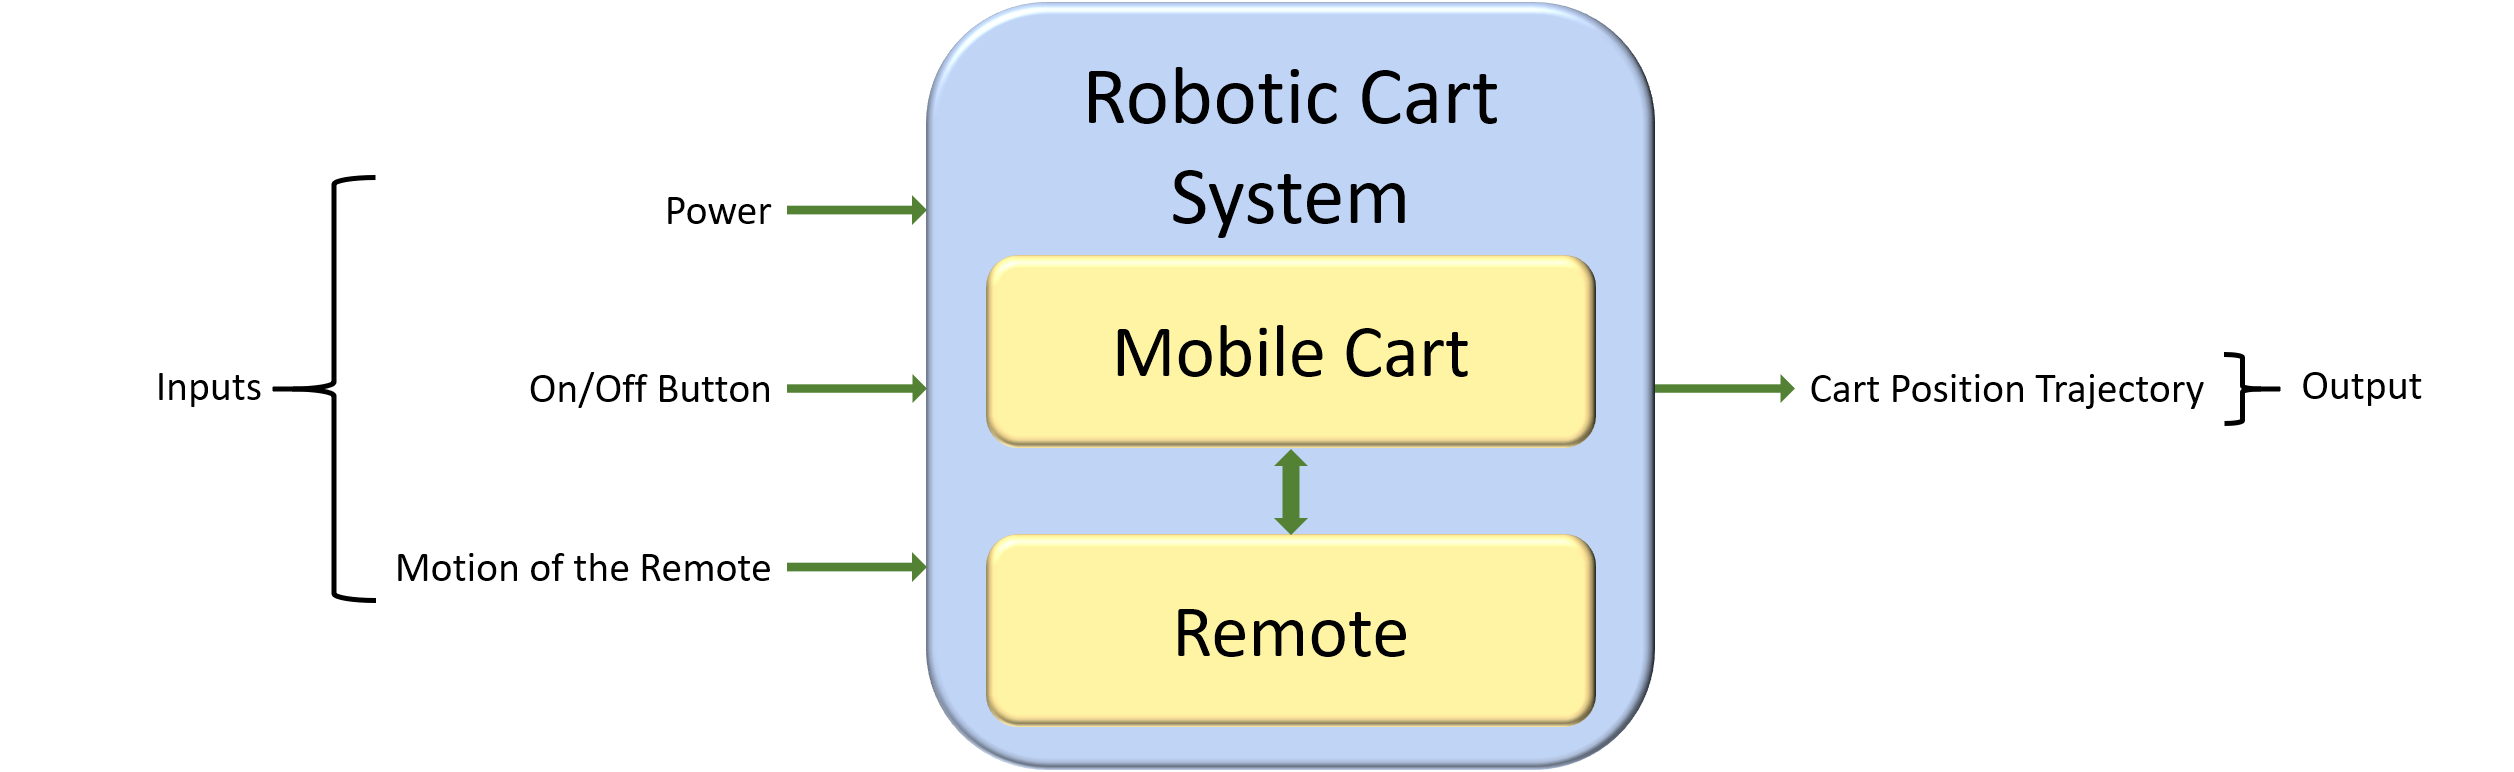
\includegraphics[width=\textwidth]{figs/img/systemBlockDiagram.png}
  \caption{System level block diagram detailing inputs and outputs to the
    robotic cart system.}
	\label{fig:sys_block_diag}
\end{figure}

\vspace*{12pt}
\noindent
The main output of the system is the position trajectory of the robotic cart in its environment. When the user moves with the remote target, the robotic cart is designed to follow the user.



%----------------------------------------------------------------------
\section{Subsystem Block Diagrams}
%----------------------------------------------------------------------
The Mobile Cart and the Remote Target subsystems are two separate operations
within the robotic cart system that run simultaneously. The two subsystems
communicate with one another by relaying radio messages between them. The first
block diagram is of the Remote Target subsystem shown in Fig.
\ref{fig:remote_block_diag}. Of the two subsystems the Remote Target is the
simplest since it only requires an XBee module attached to a 7.4V Li-Po battery
with a voltage regulation circuit since the XBee has a smaller input voltage of
3.3 volts. The two inputs for this system are the battery power and the incoming
RF messages which are passed through the RF transceiver Module and output the
outgoing RF messages.

\begin{figure}[H]
  \centering
  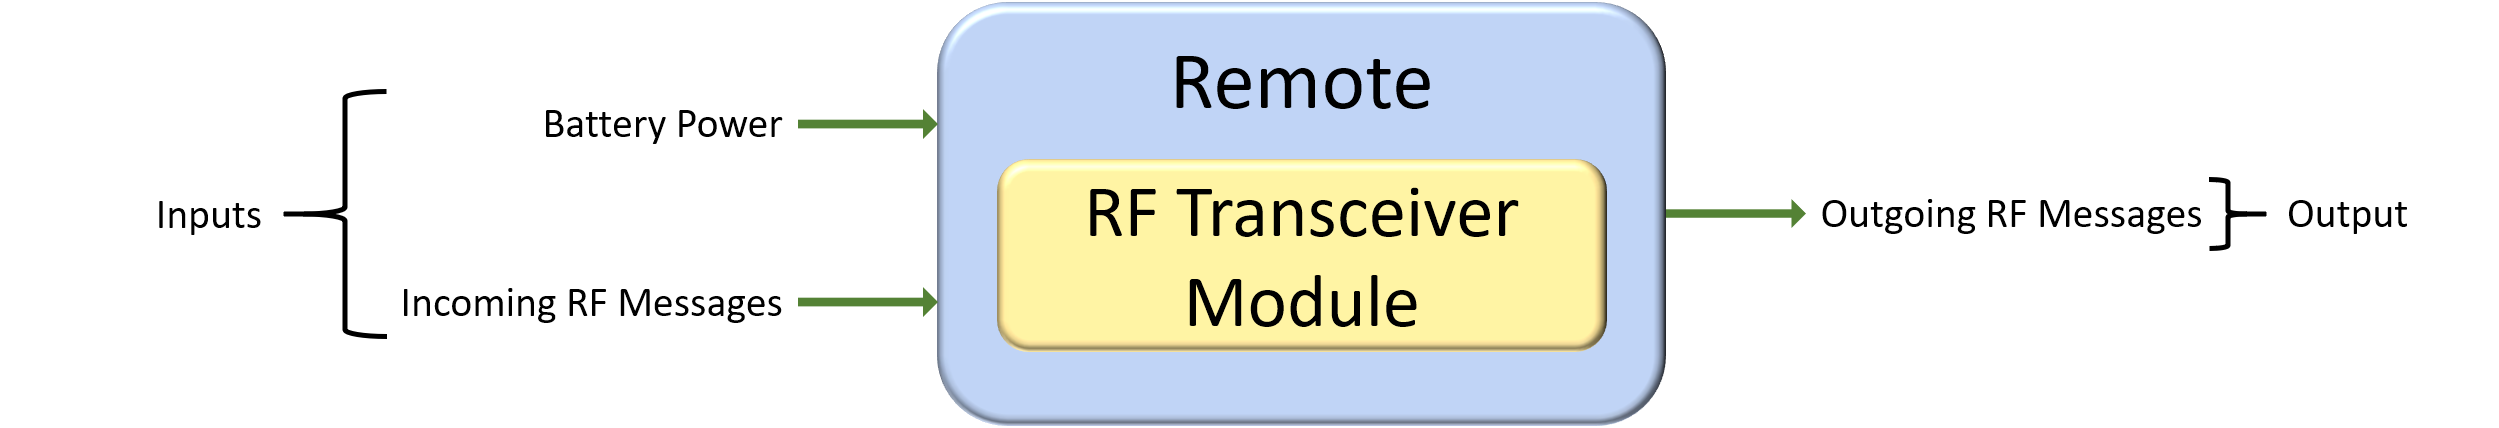
\includegraphics[width=\textwidth]{figs/img/remoteBlockDiagram.png}
  \caption{Remote Target block diagram}
  \label{fig:remote_block_diag}
\end{figure}

\vspace*{12pt}
\noindent
The Mobile Cart subsystem block diagram, shown in Fig.
\ref{fig:mobile_block_diag}, is the most complex of the two subsystems.The cart requires a power source, which will be a 7.4V, 8,000 mAh Li-Po battery since the
Li-Po works well with powering the embedded computer (BeagleBone Blue). The
power to the subsystem will be toggled by an on/off switch located on the
chassis of the robotic cart. The final input to the mobile cart subsystem is the
incoming RF signals. These incoming RF signals are passed to the direction
sensitive RF receivers which output the signals to the dual-direction
multiplexer. The dual-direction multiplexer then takes the four inputs from the
direction sensitive RF receivers and passes one output into the embedded
computer. Once the embedded computer gets these signals it can calculate the
localization and navigation algorithms and pass the information to the DC
motors.

\begin{figure}[H]
  \centering
  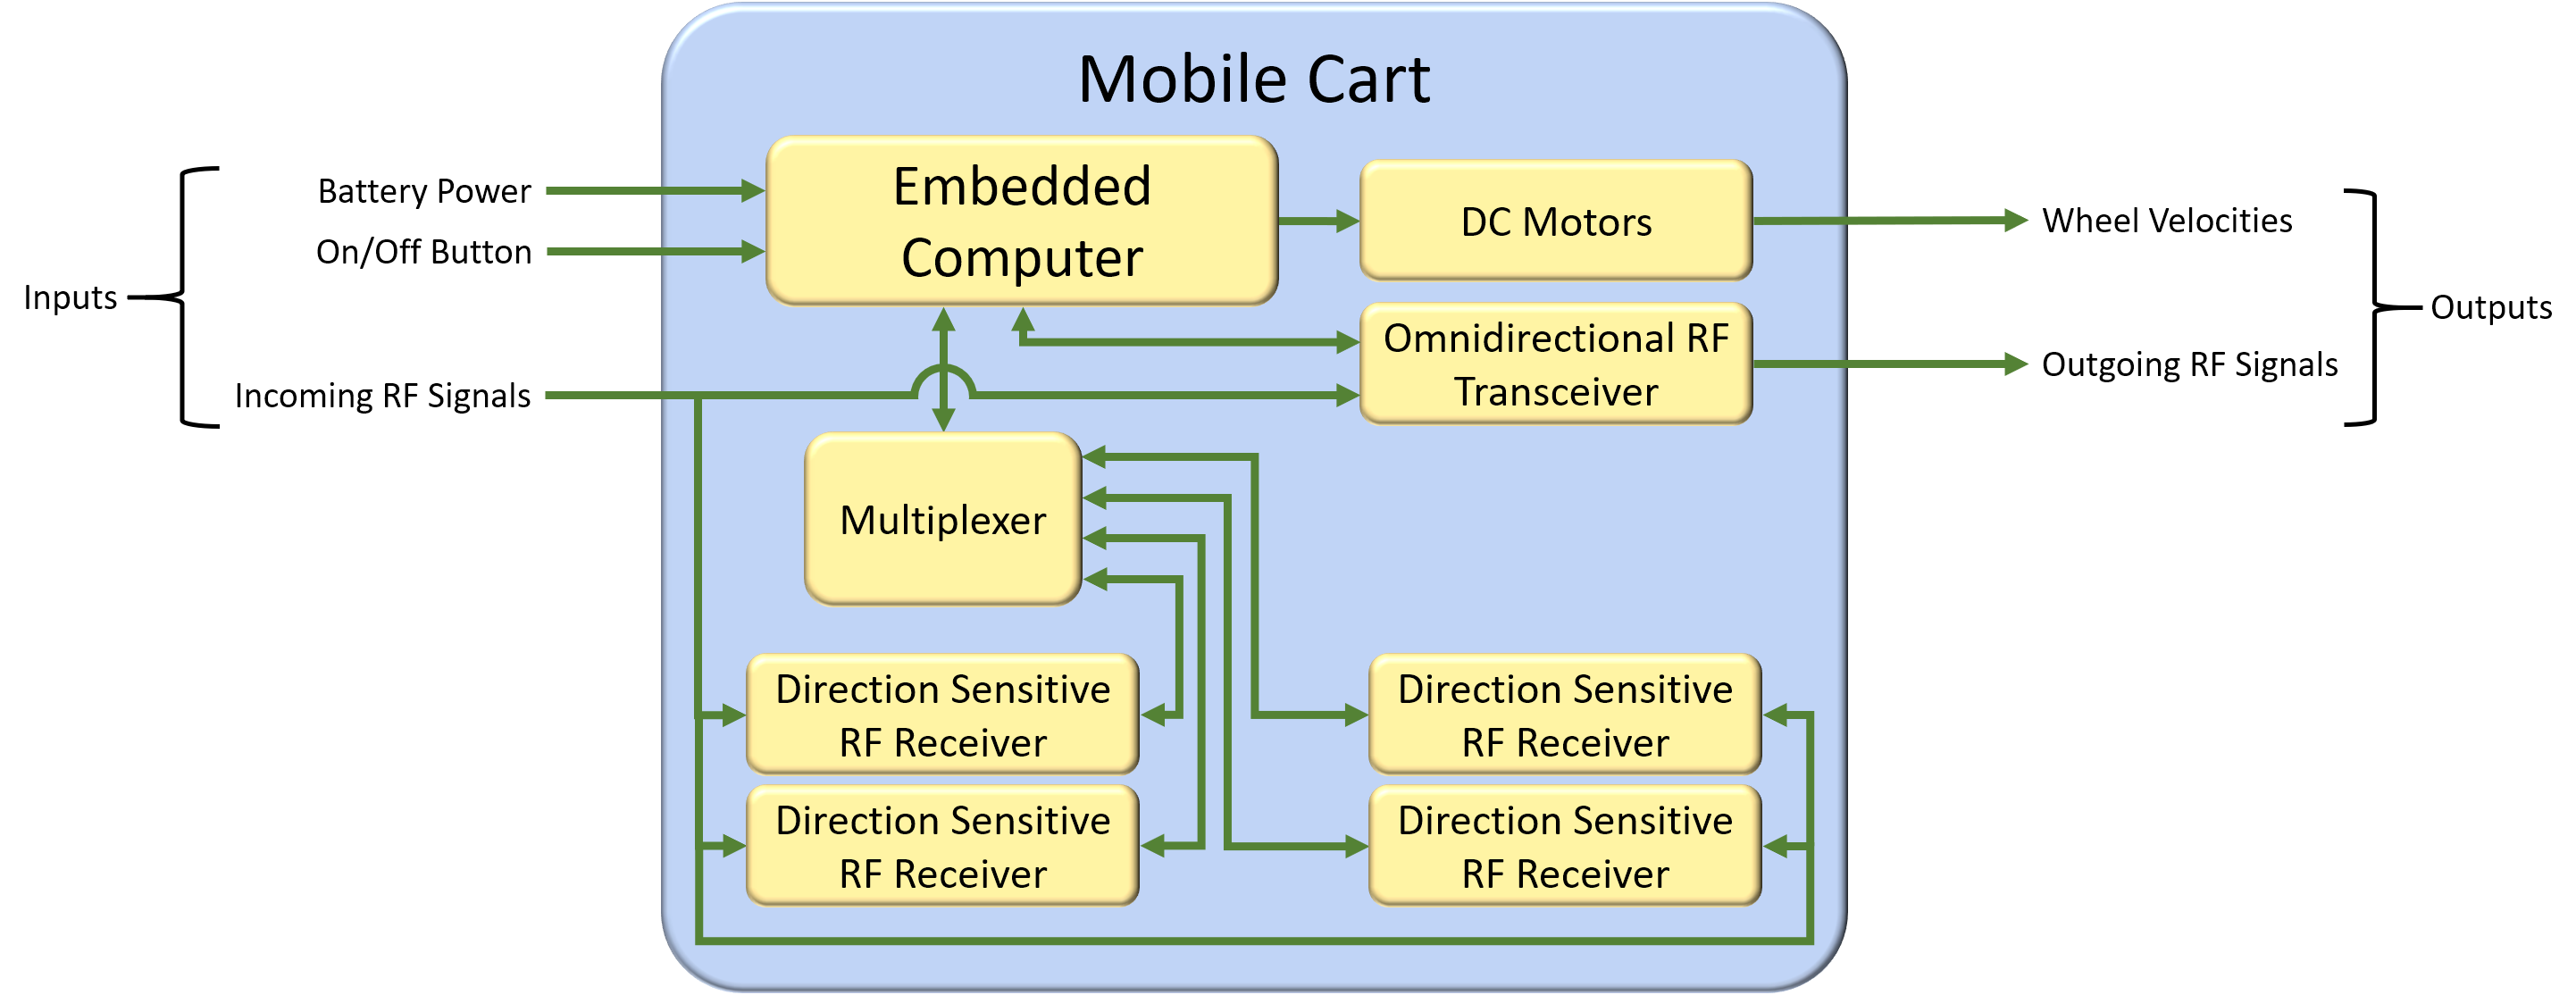
\includegraphics[width=\textwidth]{figs/img/mobileCartBlockDiagram.png}
  \caption{Block diagram showing the subsystem-level components of the proposed robotic cart.}
  \label{fig:mobile_block_diag}
\end{figure}

\vspace*{12pt}
\noindent
There are two outputs of the mobile cart subsystem. The first is the wheel velocities that move the cart and are passed from the DC motors. Lastly, the incoming RF signals are passed to our omnidirectional RF transceiver which outputs the outgoing RF signals.


%----------------------------------------------------------------------
\section{System Components}
\label{sec:System Components}
%----------------------------------------------------------------------

There are several components that are required for the mobile cart system.
Although some of these parts are available in the Bradley University laboratory,
other parts must be purchased. The parts that exist in the lab are listed in
\autoref{tab:Partslablist}. Also, \autoref{tab:Partslist} shows the list of
parts that were purchased. The parts compiled in the lists are the required
parts needed to build two smart robotic cart systems.

\begin{table}[h!]
  \centering
  \caption{Parts Available in Laboratory}
  \begin{tabular}{c|c}
      \toprule
      \textbf{Quantity} & \textbf{Parts}\\
      \toprule
      2 & Budget Bot Chassis\\
      4 & 10 uF Ceramic Capacitor\\
      4 & LM1117 Regulator\\
      8 & 9V Batteries\\
      4 & Solderable PCB Boards\\
      3 & XBee USB Adapter\\
      \bottomrule
      %\multicolumn{2}{r|}{\textbf{Total}} & \$ 562.34\\
      %\bottomrule
  \end{tabular}
  %\caption{Parts Available in Laboratory}
  \label{tab:Partslablist}
\end{table}

\begin{table}[h!]
  \centering
  \caption{Purchased parts for the Robotic Cart Project}
  \begin{tabular}{c|c|c}
    \toprule
    \textbf{Quantity} & \textbf{Parts} & \textbf{Price}\\
    \toprule
    4 & Pololu 37D Metal Gear motor 4751 & \$ 39.95\\
    12 & XBee S2C Module & \$ 23.10\\
    10 & XBee Adapter Board & \$ 4.99\\
    2 & Twotrees 4 Lead Nema 17 Stepper Motor & \$ 9.99\\
    1 & 4-Pin JST SH Connector - 20 Pack & \$ 7.99\\
    1 & 6-Pin JST SH Connector - 10 Pack & \$ 9.99\\
    1 & Aluminum Foil Tape - 2 in x 5 yd & \$ 6.05\\
    2 & Ovonic 7.4V 8000mAh LiPo Battery & \$ 40.99\\
    4 & Multiplexers & \$ 15.99\\
    \bottomrule
    \multicolumn{2}{r|}{\textbf{Total}} & \$ 562.34\\
    \bottomrule
  \end{tabular}
  %\caption{Purchased parts for the Robotic Cart Project}
  \label{tab:Partslist}
\end{table}

\vspace*{6pt}
\noindent
The main components for this project are the Budget Bot Chassis (Fig.
\ref{fig:budgetBotChassis}), the BeagleBone Blue embedded computer (Fig.
\ref{fig:beagleboneBlue}), and the XBee S2C Modules (Fig. \ref{fig:XBeeModule}).
Another major component is the reflector array that will be used to
directionally receive the RF signals from the remote target that is with the
user.

\begin{figure}
  \centering
  \begin{subfigure}[t]{0.32\linewidth}
    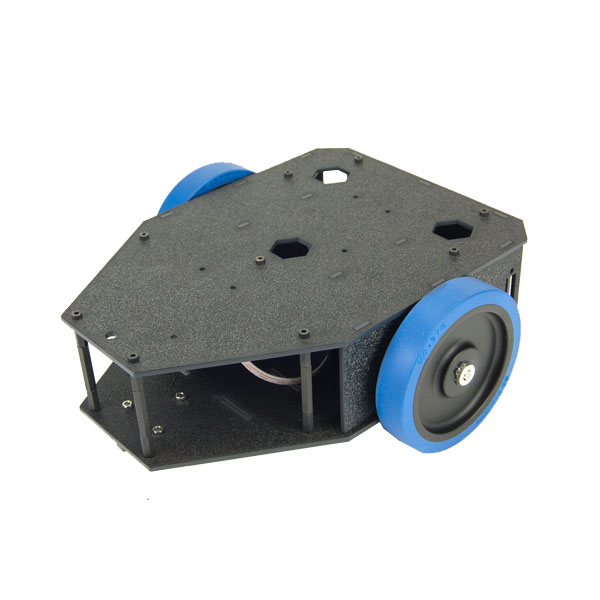
\includegraphics[width=1\linewidth]{figs/img/budgetbot_chassis}
    \captionsetup{width=\linewidth}
    \caption{Budget Bot Chassis}
    \label{fig:budgetBotChassis}
  \end{subfigure}
  \begin{subfigure}[t]{0.32\linewidth}
    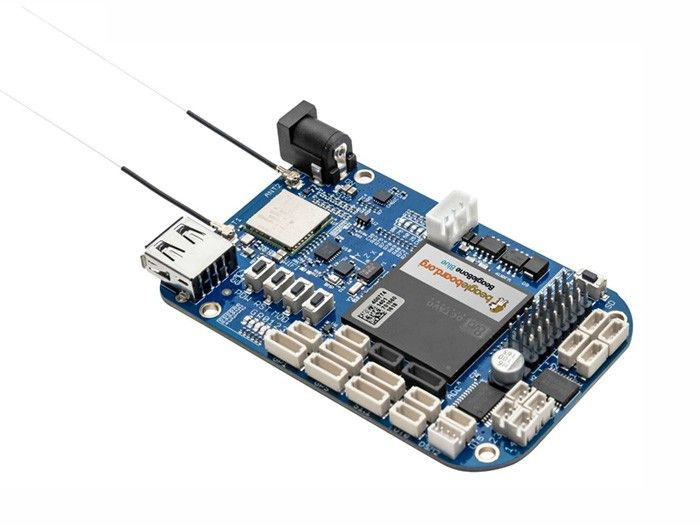
\includegraphics[width=1\linewidth]{figs/img/beaglebone_blue}
    \captionsetup{width=\linewidth}
    \caption{BeagleBone Blue}
    \label{fig:beagleboneBlue}
  \end{subfigure}
  \begin{subfigure}[t]{0.32\linewidth}
    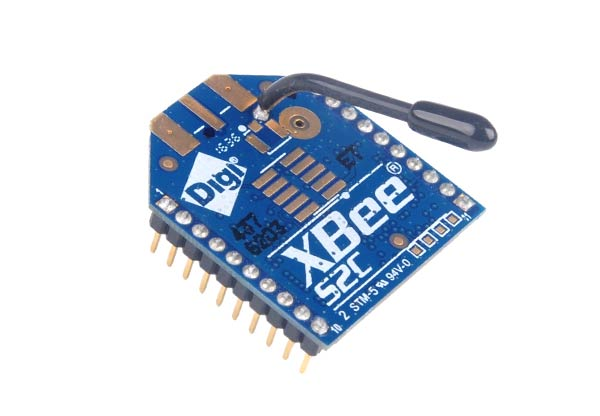
\includegraphics[width=1\linewidth]{figs/img/Xbee-S2C-Module}
    \captionsetup{width=\linewidth}
    \caption{XBee S2C Module}
    \label{fig:XBeeModule}
  \end{subfigure}
\end{figure}

\vspace*{12pt}
\noindent
The reflector array will be mounted on top of the cart with a stepper motor.
There are two reflector designs that were evaluated in this project. The first,
shown in Fig. \ref{fig:parabolodialReflector}, is a paraboloidal reflector which
maximizes the signal strength of the signals that come into the reflector
perpendicularly. Since the remote will be carried by the user, it is likely that
it will be positioned at a higher altitude than the reflector array. The
paraboloidal reflector design may not be able to pick up the signals from the
remote as well because of this. %
%
%
\begin{figure}
  \centering
  \begin{subfigure}[t]{0.5\linewidth}
    \centering
    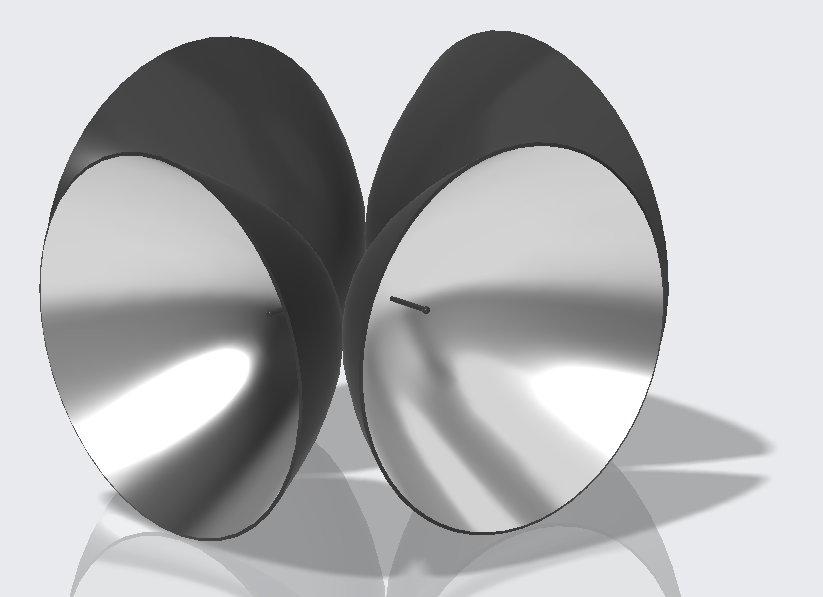
\includegraphics[height=2in\linewidth]{figs/img/paraboloidalReflector}
    \captionsetup{width=\linewidth, justification=raggedright}
    \caption{Paraboloidal Reflector Model}
    \label{fig:parabolodialReflector}
  \end{subfigure}
  \begin{subfigure}[t]{0.4\linewidth}
    \centering
    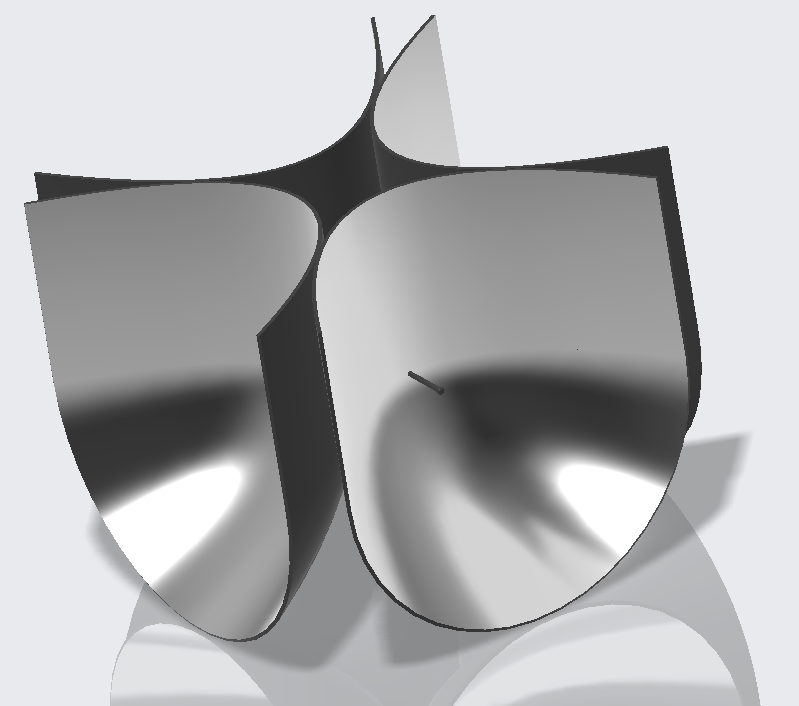
\includegraphics[height=2in\linewidth]{figs/img/parabolicReflector}
    \captionsetup{width=\linewidth, justification=raggedright}
    \caption{Combined Parabolic/Paraboloidal Reflector}
    \label{fig:parabolicReflector1}
  \end{subfigure}
\end{figure}
%
To solve this problem, a combination parabolic/paraboloidal reflector was
designed, as shown in Fig. \ref{fig:parabolicReflector1}. The lower half of this
reflector is paraboloidal in shape to limit the signals coming from below. The
upper part of the reflector is strictly parabolic. This shape focuses the
signals in the horizontal plane, but allows signals from above to still be
received. The plan is to construct both of these reflector designs by 3D
printing the frames, then lining them with reflective foil tape. Both models
will then be tested to determine which design works better.


%----------------------------------------------------------------------
\section{Operation of Robotic Cart System}
\label{sec:Operation of Robotic Cart System}
%----------------------------------------------------------------------
The mobile cart was controlled by a central embedded computer which is the BeagleBone Blue since it is ideal in robotics control. Two DC motors were used to drive wheels and move the cart. Five XBee modules on the cart were used to allow communication with the remote target. One of these radio sensors was mounted on top of the cart to broadcast in all directions. The other four sensors were placed inside parabolic reflectors at right angles to each other. This sensor array was mounted on a stepper motor to allow rotation.


%%% Local Variables:
%%% mode: latex
%%% TeX-master: "../finalReport"
%%% End:

%======================================================================
\chapter{Customized Reflector Array}
\label{ch: Chapter3}
%======================================================================

%----------------------------------------------------------------------
\section{Reflector Design}
%----------------------------------------------------------------------
The XBee RF modules that were used detect signals from any direction. For this project, however, it is desired to have differences in the received signals based on the angle from which the signal is coming. To accomplish this, two different models of reflector arrays were designed and constructed. 

\subsection{Purely Paraboloidal Reflector}
The first design, shown in \autoref{fig:paraboloidalReflector}, uses a reflector with a purely paraboloidal shape. This shape was selected since all signals entering the reflector parallel to the axis of the reflector will pass through the focus of the paraboloid. By mounting the XBee such that the center of the antenna coincides with the focus of the paraboloid, the signal strength of the signals entering parallel to the axis will be maximized.
\begin{figure}
    \centering
    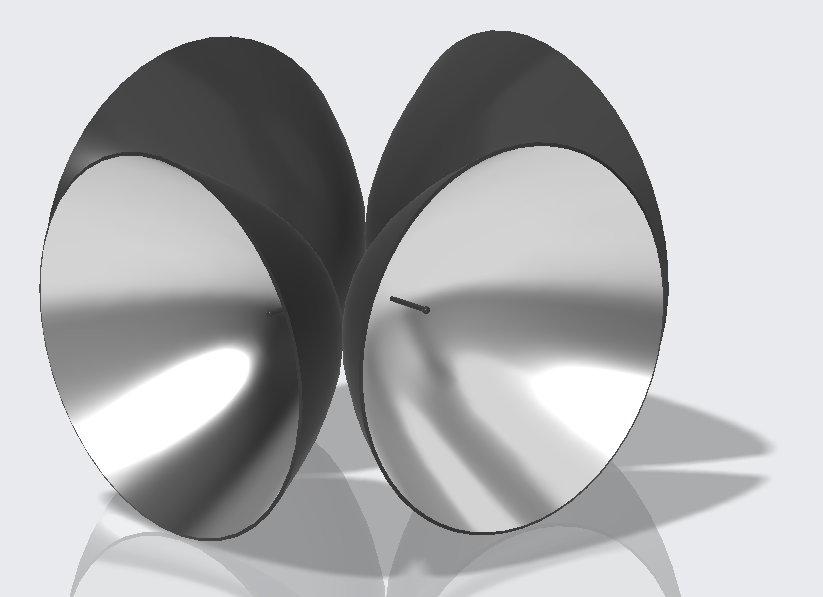
\includegraphics[width=3.5in]{figs/img/paraboloidalReflector.png}
    \caption{Purely Paraboloidal Reflector Array}
    \label{fig:paraboloidalReflector}
\end{figure}

\subsection{Combined Parabolic/Paraboloidal Reflector}
The second design, shown in \autoref{fig:parabolicReflector}, is the same on the lower half as the first design. However, the upper half is simply a surface where the horizontal cross-section is a parabola. The purpose for this design is similar to that of the first design, but the parabolic shape on the top will allow stronger detected signal strength of signals coming from above the reflector. Since the remote will be held by a person, it will generally be above the robot. The parabolic/paraboloidal reflector design is intended to allow better reception of signals from above.
\begin{figure}
    \centering
    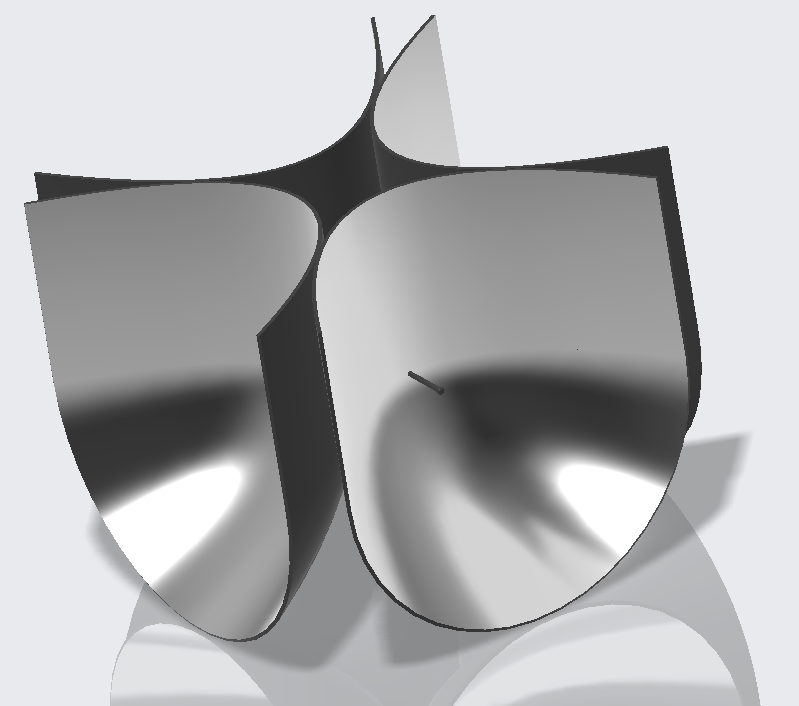
\includegraphics[width=3.5in]{figs/img/parabolicReflector.png}
    \caption{Parabolic/Paraboloidal Reflector Array}
    \label{fig:parabolicReflector}
\end{figure}

%----------------------------------------------------------------------
\section{Reflector Construction}
%----------------------------------------------------------------------
The reflector dishes were created using a 3D printer. After printing, the dishes were lined with reflective foil tape


%----------------------------------------------------------------------
\section{Experimental Results}
%----------------------------------------------------------------------


%%% Local Variables:
%%% mode: latex
%%% TeX-master: "../finalReportMainV1"
%%% End:
%======================================================================
\chapter{Localization and Navigation}
\label{ch: Chapter4}
%======================================================================

\todo[inline]{Add an introductory paragraph. For example, ``In this Chapter, we
  illustrate localization and navigation algorithms for the mobile cart to operate in an
  indoor/outdoor environment. For that, we first model the proposed robotic cart
  as a differential drive mobile robot (DDMR). The position of the cart is then
  determined using a localization algorithm. $\ldots$''}

%----------------------------------------------------------------------
\section{Robot Model}\label{sec:robotModel}
%----------------------------------------------------------------------
The robot used in this project was a differential drive mobile robot, which has
two drive wheels and a caster wheel for balance. The robot turns by applying
different speeds to the left and right wheels. As shown in Fig.
\ref{fig:robotGeometry}, the radius of the wheels is $R$, and the distance
between the wheels is $L$. The pose of the robot is given by the $x$-coordinate
($x$), the $y$-coordinate ($y$), and the orientation, ($\theta$), as shown in
Fig. \ref{fig:robotPose}. %
%
\begin{figure}
    \centering
    \begin{subfigure}{0.3\textwidth}
        \centering
        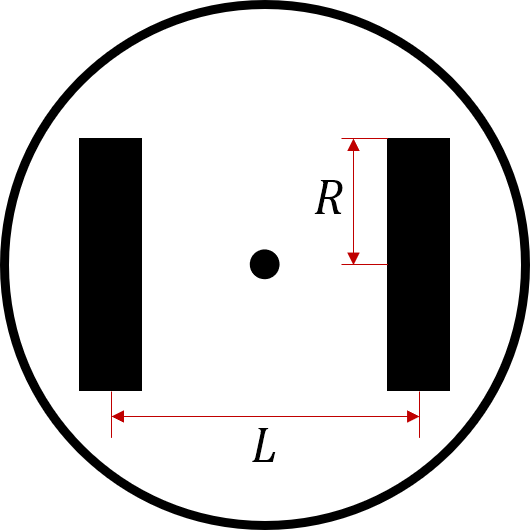
\includegraphics[width=0.9\textwidth]{figs/img/robotGeometry.png}
        \caption{Robot Geometry}
        \label{fig:robotGeometry}
    \end{subfigure}%
    \begin{subfigure}{0.7\textwidth}
        \centering
        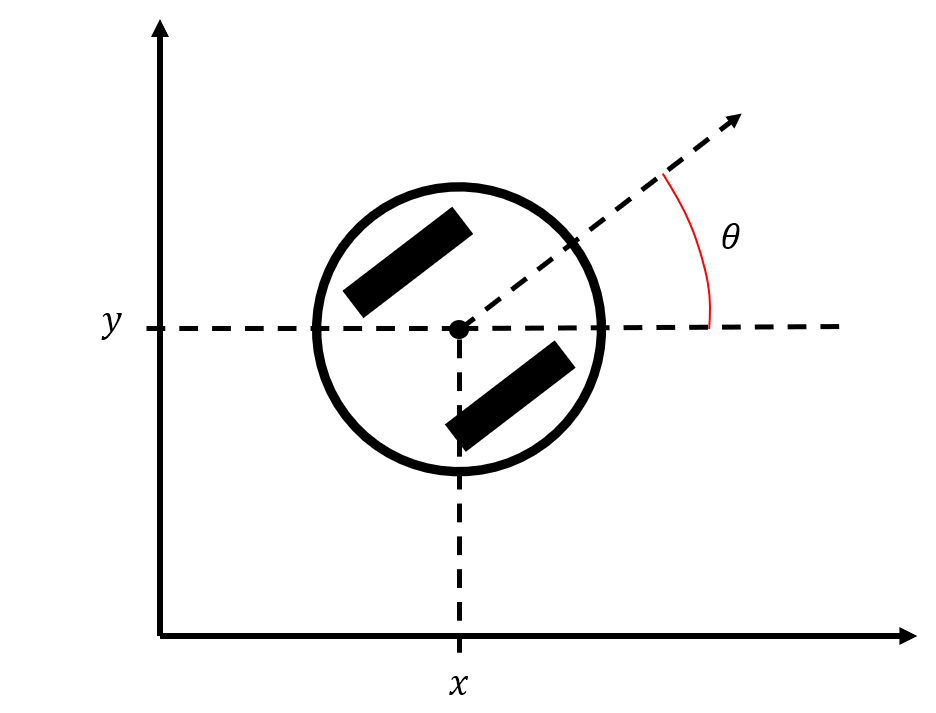
\includegraphics[width=0.9\textwidth]{figs/img/robotPose.png}
        \caption{Robot Pose}
        \label{fig:robotPose}
    \end{subfigure}
    \caption{Robot Model Parameters}
    \label{fig:robotModelParameters}
\end{figure}
%

Generally the robot is controlled by commanding a linear and angular speed ($v$ and $\omega$, respectively). These speeds must be converted into left and right wheel speeds. The following equations are used to calculate the angular left and right wheel speeds ($\omega_l$ and $\omega_r$, respectively):
$$\omega_l = \left(v - \omega\frac{L}{2}\right)\frac{1}{R}$$
$$\omega_r = \left(v + \omega\frac{L}{2}\right)\frac{1}{R}$$
To control DC motors in this way, the relationship between duty cycle and angular speed must be determined. Then the duty cycles to apply to the wheels can be calculated for the commanded $v$ and $\omega$.

%----------------------------------------------------------------------
\section{Localization Algorithm}
%----------------------------------------------------------------------
The localization algorithm is used to estimate the position of the remote with respect to the robot's local coordinate system. First the omnidirectional transceiver on top of the reflectors sends a signal strength request to the remote. The remote then replies with a message containing the strength of the signal it just received. This reply is detected by the receivers inside the reflectors as well as the omnidirectional transceiver. The strength detected by each of the directional receivers and the strength contained in the reply are then recorded. At this point, the entire reflector array is rotated 9\textdegree, and this process is repeated. The robot continues taking measurements in this way until the reflectors have been rotated one quarter turn. Since there are four reflectors at 90\textdegree to each other, a strength measurement has been recorded for every 9\textdegree increment around the robot. The angle of the remote is then estimated as the direction from which the strongest signal was received. The distance to the remote is calculated using the free-space path loss formula. The direction of reflector rotation is then reversed since the wires connecting the RF modules in the reflectors prevent the reflector from freely spinning. A flowchart of this algorithm is shown in Fig. \ref{fig:localizationAlgoFlowchart}.
\begin{figure}
    \centering
    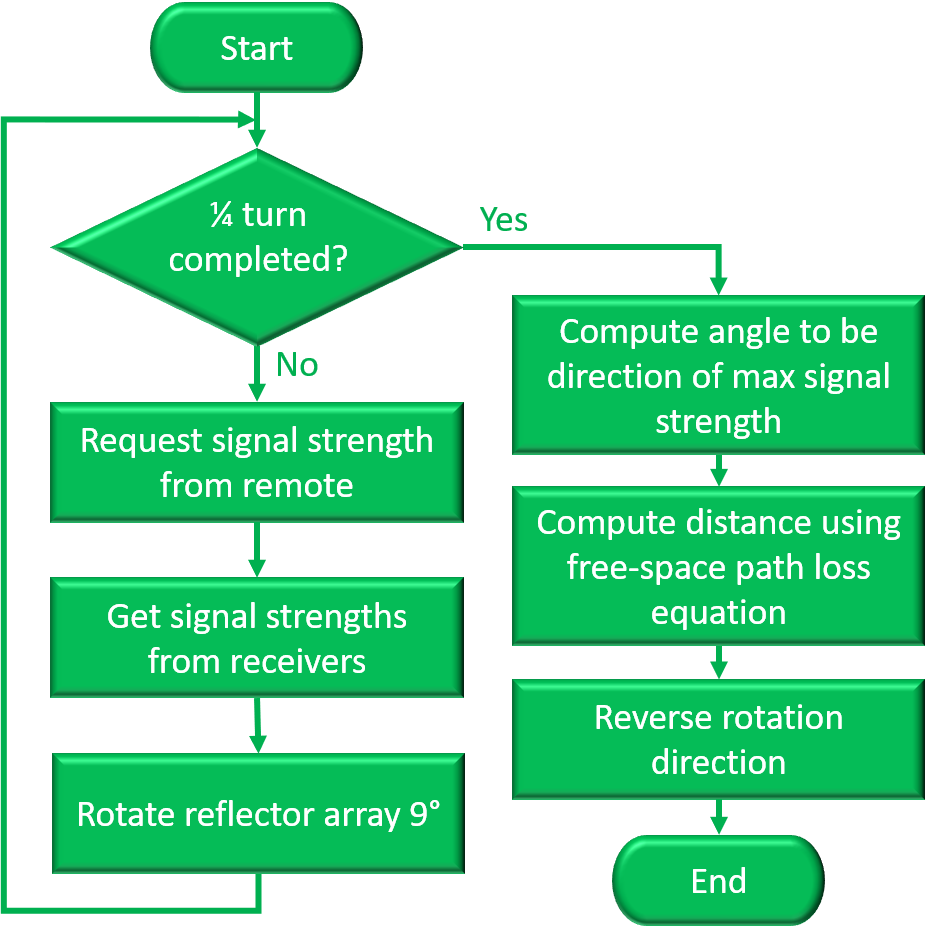
\includegraphics[width=3.5in]{figs/img/localizationAlgoFlowchart.png}
    \caption{Flowchart of Localization Algorithm}
    \label{fig:localizationAlgoFlowchart}
\end{figure}

%----------------------------------------------------------------------
\section{Navigation Algorithm}
%----------------------------------------------------------------------
The navigation algorithm is used to drive the robot toward the remote. The inputs to the navigation algorithm are the angle to the remote ($\theta_r$) and the distance to the remote ($d_r$). A target point is then calculated as the point that is in the same direction as the remote, but closer to the robot by a fixed following distance ($d_{follow}$), as shown in Fig. \ref{fig:navAlgoDiagram}. The distance to the target point is calculated as $d_{tgt} = d_r - d_{follow}$, and the angle to the target point is $\theta_{tgt} = \theta_r$. The linear and angular speeds of the robot ($v$ and $\omega$, respectively) are then calculated using proportional control by the following equations:
$$v = K_vd_{tgt}$$
$$\omega = K_\omega\theta_{tgt}$$
The appropriate duty cycles are then calculated as specified in section \ref{sec:robotModel} and applied to the wheel motors.
\begin{figure}
    \centering
    \begin{subfigure}{0.45\textwidth}
        \centering
        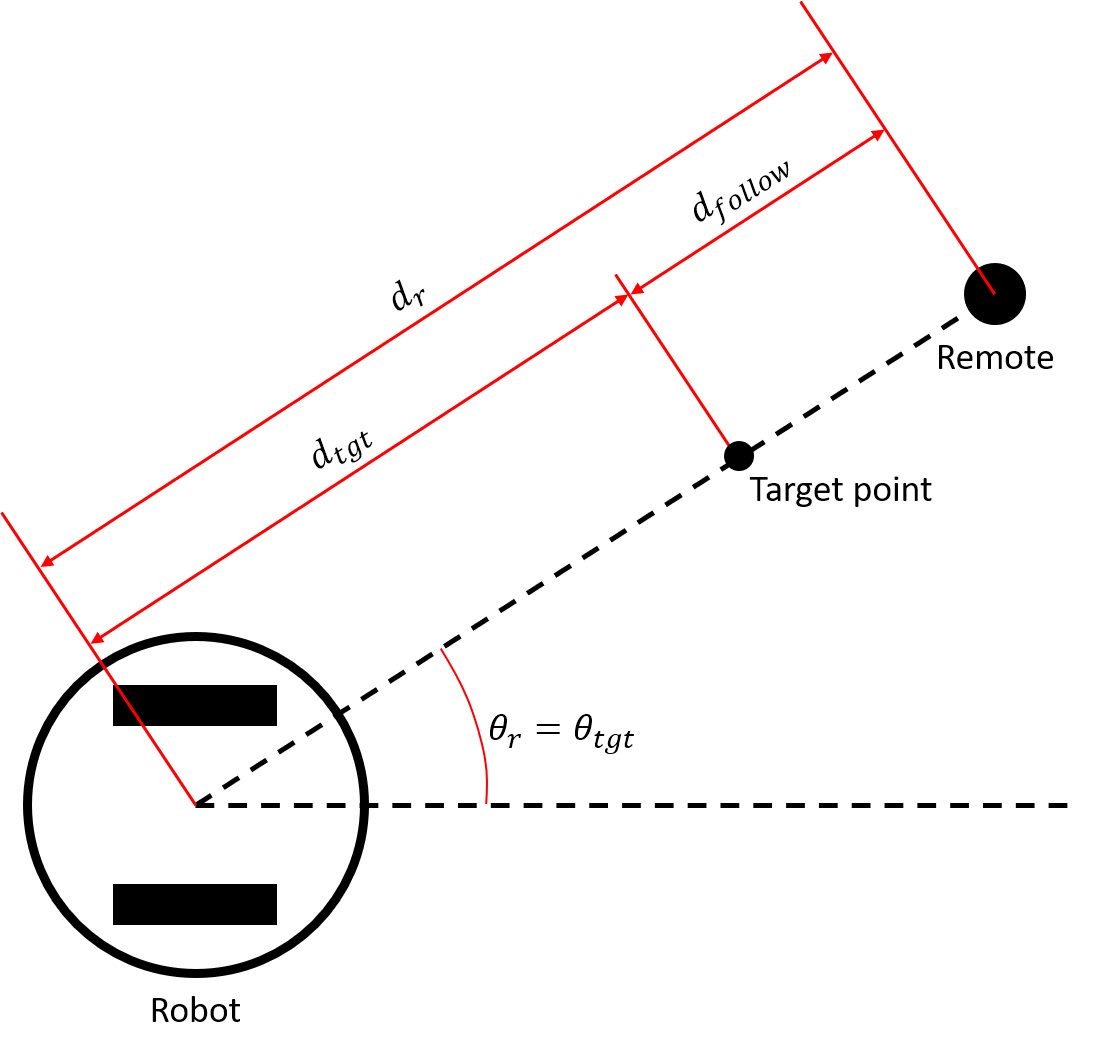
\includegraphics[width=0.95\textwidth]{figs/img/navAlgoDiagram.png}
        \caption{Target Point Diagram}
        \label{fig:navAlgoDiagram}
    \end{subfigure}%
    \begin{subfigure}{0.55\textwidth}
        \centering
        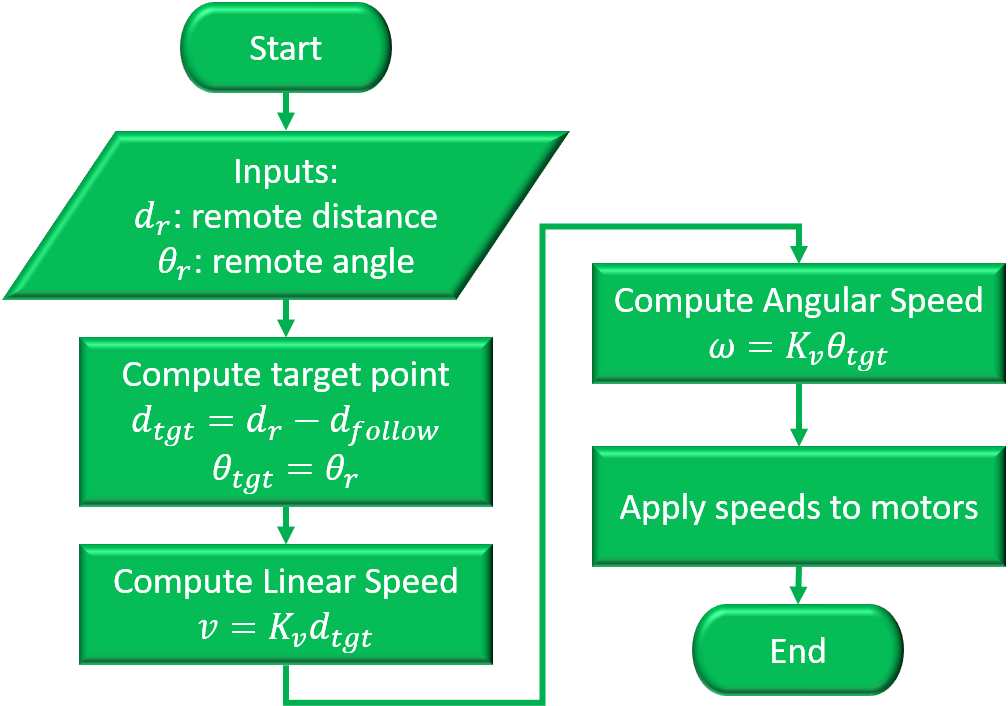
\includegraphics[width=0.95\textwidth]{figs/img/navigationAlgoFlowchart.png}
        \caption{Flowchart}
        \label{fig:navAlgoFlowchart}
    \end{subfigure}
    \caption{Navigation Algorithm Details}
    \label{fig:navAlgoDetails}
\end{figure}

%%% Local Variables:
%%% mode: latex
%%% TeX-master: "../finalReport"
%%% End:

%======================================================================
\chapter{Implementation}
\label{ch: Chapter5}
%======================================================================

%----------------------------------------------------------------------
\section{Robot Assembly}
%----------------------------------------------------------------------



%----------------------------------------------------------------------
\section{Code Trial and Implementation}
%----------------------------------------------------------------------



%----------------------------------------------------------------------
\section{Experimental Results}
%----------------------------------------------------------------------


%%% Local Variables:
%%% mode: latex
%%% TeX-master: "../finalReportMainV1"
%%% End:
%======================================================================
\chapter{Conclusion and Future Work}
\label{ch: Chapter6}
%======================================================================

%----------------------------------------------------------------------
\section{Conclusion}
%----------------------------------------------------------------------


%----------------------------------------------------------------------
\section{Future Work}
%----------------------------------------------------------------------


%%% Local Variables:
%%% mode: latex
%%% TeX-master: "../finalReportMainV1"
%%% End:

% %----------------------------------------------------------------------
% % APPENDICES
% %---------------------------------------------------------------------- 
\appendix
% % Designate with \appendix declaration which just changes numbering style 
% % from here on
% % Add a title page before the appendices and a line in the Table of Contents
\addcontentsline{toc}{chapter}{APPENDICES} 
% %

% %======================================================================
\chapter{Modeling in CoppeliaSim}
\label{ch: coppSimModeling}
%======================================================================

%----------------------------------------------------------------------
\section{Problem Statement}
%----------------------------------------------------------------------
It is important to be able to simulate a robot's behavior before using the
actual robot to help find unexpected behaviors. CoppeliaSim is commercial robot
simulation software with the ability to simulate a robot that would operate in
exactly the way it would happen with a real robot. However, the robot of
interest is not currently included in CoppeliaSim's library that leads to
creating a model of the robot and simulating it before practical implementation.
The following sections explain how to model the Runt Rover robot in CoppeliaSim.

%----------------------------------------------------------------------
\section{Dimensions and 3D Modeling}
%----------------------------------------------------------------------
The Runt Rover robot is geometrically simple, with only a few dimensions being necessary to model the shape of the body and wheels. The dimensions used in this guide are shown in Fig. \ref{fig:runtRoverDims}

\begin{figure}
    \centering
    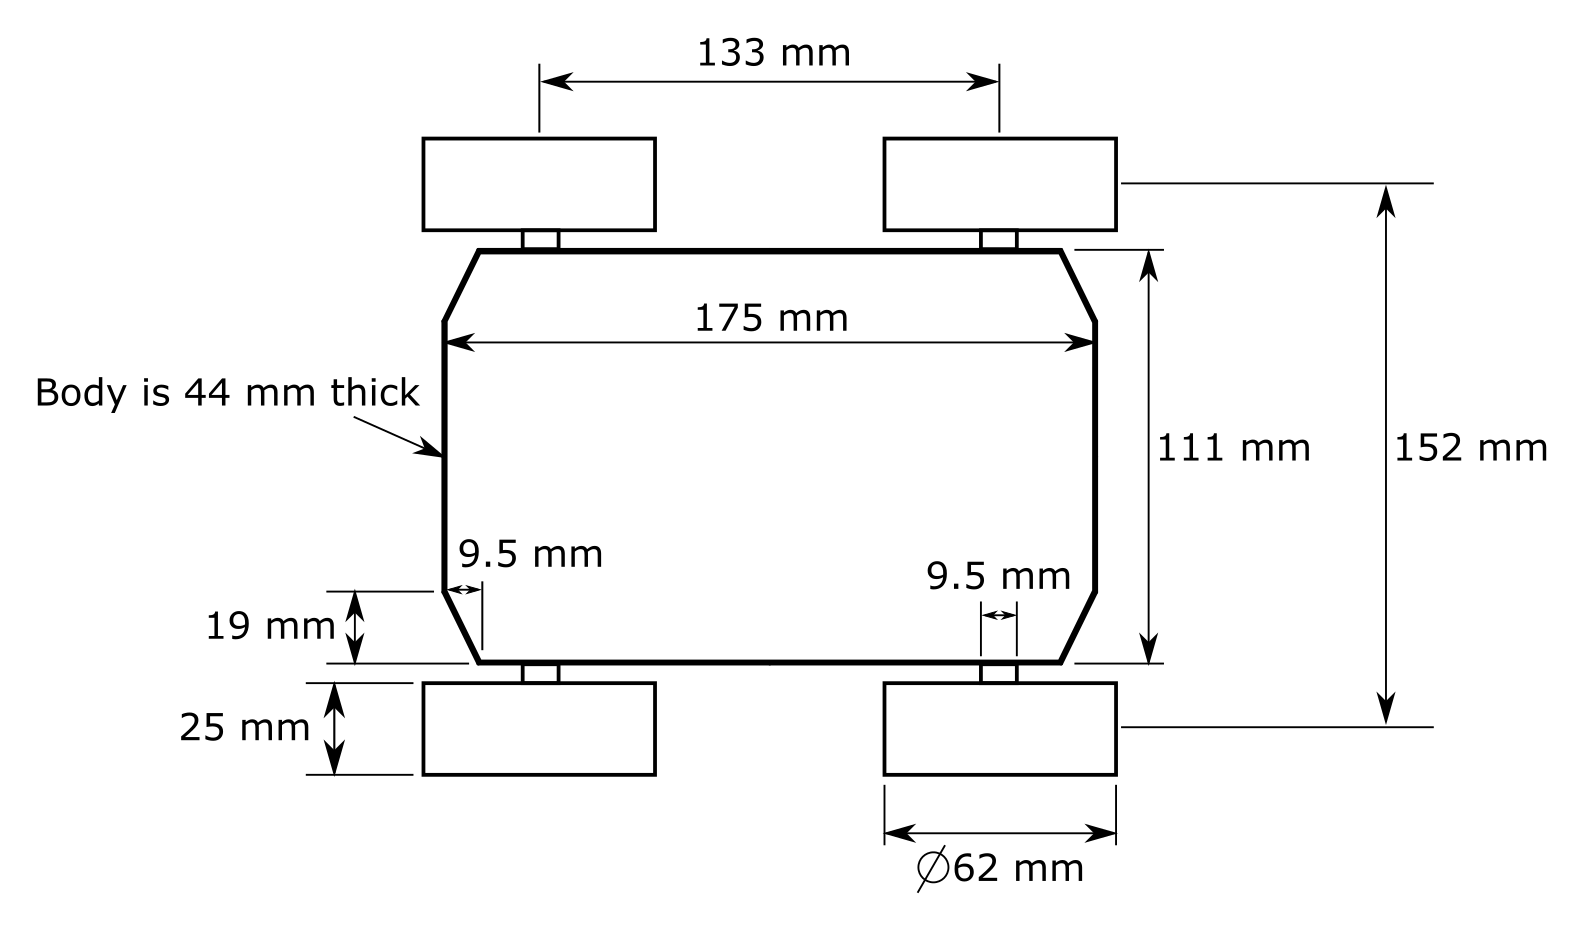
\includegraphics[width=3.5in]{figs/img/runtRoverDimensions}
    \caption{Dimensions of the Runt Rover Robot}
    \label{fig:runtRoverDims}
\end{figure}

The final 3D models are shown in Fig. \ref{fig:runtRoverModels}. An arrow was placed on the body to indicate orientation during simulation.

\begin{figure}
    \centering
    \begin{subfigure}[b]{0.6\textwidth}
        \centering
        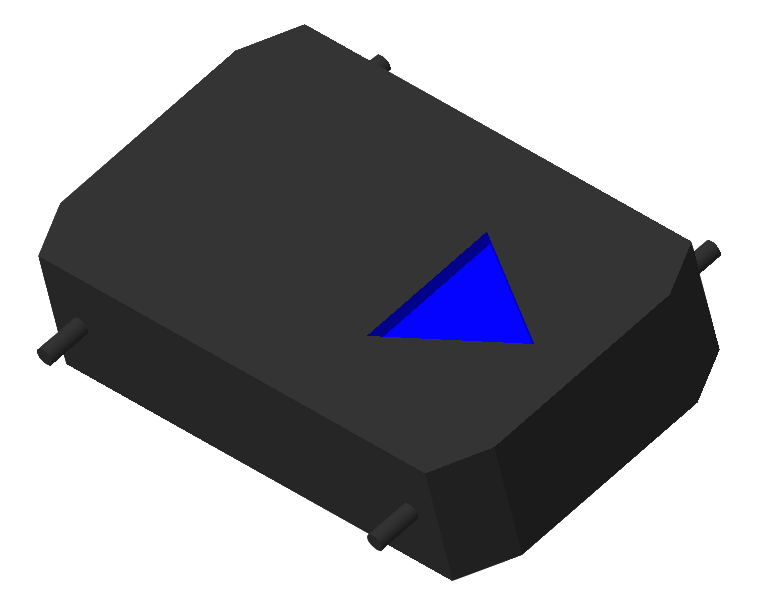
\includegraphics[width=\textwidth]{figs/img/runtRoverChassis}
        \caption{Chassis}
        \label{fig:runtRoverChassis}
    \end{subfigure}
    \hfill
    \begin{subfigure}[b]{0.3\textwidth}
        \centering
        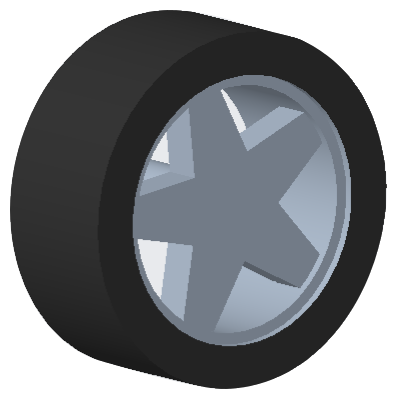
\includegraphics[width=\textwidth]{figs/img/runtRoverWheel}
        \caption{Wheel}
        \label{fig:runtRoverWheel}
    \end{subfigure}
    \caption{Modeled Parts}
    \label{fig:runtRoverModels}
\end{figure}

%----------------------------------------------------------------------
\section{Importing Models}
%----------------------------------------------------------------------
The next step is to import the 3D models into CoppeliaSim. This is accomplished using File \textgreater \ Import \textgreater \ Mesh. If the models were dimensioned in millimeters, the scale must be changed to 0.001 since CoppeliaSim uses meters. Since there are multiple colors in the models, there will be multiple shapes in CoppeliaSim. These can be grouped by dragging one shape onto another. Also, the shapes can be renamed. In modeling the Runt Rover, one chassis and four wheels are needed. The wheels must be placed in the correct locations on the axles.

%----------------------------------------------------------------------
\section{Adding Motors}
%----------------------------------------------------------------------
The robot can be given motors by means of revolute joints. These can be added using Add \textgreater \ Joint \textgreater \ Revolute. For the Runt Rover, one revolute joint was placed at each wheel. The joints should be named according to the wheel location since their names are used to interface the robot with Matlab. These joints are then made invisible by moving them to visibility layer 10. This is achieved in the Object Common Properties dialog box. The joints can be viewed by turning on visibility for layer 10 using the Layers dialog box. In the Object Properties dialog box, there is a button to open the Dynamic Properties dialog box. In this box, make sure the ``Motor enabled'' checkbox is enabled.

%----------------------------------------------------------------------
\section{Dynamic Shapes}
%----------------------------------------------------------------------
The 3D models do not have any dynamic properties within CoppeliaSim. It is recommended to use primitive shapes for the dynamic properties to reduce computation during simulation. For the Runt Rover, the wheels can be dynamically represented as cylinders, and the chassis can be dynamically represented as a cuboid. To add a primitive cylinder, use Add \textgreater \ Primitive Shape \textgreater \ Cylinder, and specify the size to be the same as a wheel. To add a cuboid, use Add \textgreater \ Primitive Shape \textgreater \ Cuboid, and specify the size to be the same as the chassis. These bodies must now be configured with the appropriate dynamic properties.

In the dynamic properties dialog box, make sure the ``Body is respondable'' checkbox is enabled, and enable the first four checkboxes and disable the last four checkboxes in the local respondable mask. Repeat this process on all of the dynamic shapes, alternating between selecting the first four and selecting the last four checkboxes in the local respondable mask. To give the robot mass and inertia, make sure the ``Body is dynamic'' checkbox is enabled, and click the ``Compute mass and inertia'' button. These dynamic shapes should be named according to the parts they represent (FrontLeftWheelDyn, for example). In the Object Common Properties dialog box, assign the dynamic shapes to visibility layer 9 to make them invisible.

%----------------------------------------------------------------------
\section{Linkage}
%----------------------------------------------------------------------
Now it is time to link everything together into one robot. First assign each graphical shape to its corresponding dynamic shape by dragging and dropping it onto the dynamic shape. Then assign the dynamic shapes for the wheels to the corresponding revolute joints in the same way. Finally, assign the revolute joints to the dynamic chassis. The name of the dynamic chassis is the name that will be used to interface with Matlab, so change it to ``RuntRover.'' Assign this shape to be the model base in the Object Common Properties dialog box. To make the bounding box the correct size, select the revolute joints and enable the ``Ignored by model bounding box'' and the ``Invisible during selection'' checkboxes in the Object Common Properties dialog box. Now enable the ``Select base of model instead'' checkbox for each of the visible objects. This allows us to select the entire robot by clicking on any part.

%----------------------------------------------------------------------
\section{Saving the Model}
%----------------------------------------------------------------------
To save this model, go to File \textgreater \ Save model as \textgreater \ CoppeliaSim model. The default location should be in the CoppeliaSim models directory. Create a new directory to contain your models and save the model within that directory. Your model will now be available in the CoppeliaSim library.


%%% Local Variables:
%%% mode: latex
%%% TeX-master: "../finalReport"
%%% End:

% \input{parts/B-simulation.tex}
% %\input{parts/C-USB.tex}
% \input{parts/D-RP.tex}
% \input{parts/E-ADP.tex}
% \input{parts/tutorial.tex}

% %----------------------------------------------------------------------
% % END MATERIAL
% %----------------------------------------------------------------------

% % B I B L I O G R A P H Y
% % -----------------------
% %
% % The following statement selects the style to use for references.  It controls the sort order of the entries in the bibliography and also the formatting for the in-text labels.
% \bibliographystyle{plain}
% % This specifies the location of the file containing the bibliographic information.  
% % It assumes you're using BibTeX (if not, why not?).
% \ifthenelse{\boolean{PrintVersion}}{
% \cleardoublepage % This is needed if the book class is used, to place the anchor in the correct page,
%                  % because the bibliography will start on its own page.
% }{
% \clearpage       % Use \clearpage instead if the document class uses the "oneside" argument
% }
% \phantomsection  % With hyperref package, enables hyperlinking from the table of contents to bibliography             
% % The following statement causes the title "References" to be used for the bibliography section:
% % \renewcommand*{\bibname}{References}
% Bibliography 
\renewcommand{\bibname}{Bibliography}

% Add the References to the Table of Contents
\addcontentsline{toc}{chapter}{\textbf{References}}

\bibliographystyle{IEEEtran}
\bibliography{bib/references.bib}
% Tip 5: You can create multiple .bib files to organize your references. 
% Just list them all in the \bibliogaphy command, separated by commas (no spaces).


%----------------------------------------------------------------------
\end{document}
%======================================================================



%%% Local Variables: 
%%% mode: latex
%%% TeX-master: t
%%% End: 
